\chapter{Kvante-logiske porter}

Beregninger i en klassisk datamaskin blir gjort av logiske porter som tar inn en eller flere bit og gir ut en eller flere bit som svar. For eksempel tar en AND-port inn to bit og gir ut svaret 1 dersom begge inn-bitene er 1, ellers gir den ut svaret 0. Tilsvarende blir beregninger i en kvantedatamaskin gjort av kvante-logiske porter som tar inn en eller flere qubit og gir ut en eller flere qubit som svar. Likhetene mellom de to typer datamaskiner er altså store, men vi skal etter hvert se at kombinasjonen av at en qubit kan være i en superposisjon mellom 0 og 1 og at to eller flere qubit kan være sammenfiltret gir kvantedatamaskinen muligheter som går langt utover det klassiske datamaskiner har.

\section{Logiske porter og boolsk algebra}
På grunn av den klare analogien med vanlige logiske porter er det nyttig å ha dette friskt i minne når vi skal studere kvante-logiske porter. Derfor gir jeg et kort overblikk av klassiske logiske porter og hvordan de kan kombineres før jeg introduserer den kvantemekaniske versjonen. 

\subsection{Boolsk algebra}
Matematikken som brukes for å analysere logiske porter\footnote{Ofte brukes begrepet operasjoner i stedet for porter, spesielt når man snakker om boolsk algebra på et mer abstrakt nivå. Det er et en-til-en forhold mellom operasjonene i boolsk algebra og logiske porter anvendt i logiske kretser så distinksjonen mellom operasjoner og porter er ikke viktig.} og nettverk av slike er boolsk algebra. Boolsk algebra er en enkel algebra som opererer på variabler som kun kan ha to mulig verdier: SANT eller USANT. I en datamaskin assosieres SANT med bit-verdien 1 og USANT med bit-verdien 0, og i det videre vil jeg bruke 1 og 0 som de mulige verdiene til de boolske variablene. De grunnleggende regneoperasjonene i den boolske algebraen er:

\subsubsection{NOT (symbol $\neg$)}
NOT er en port/operasjon som tar inn en bit og gir ut en bit. En NOT-port vil alltid endre bit-verdien til det motsatte som vist i sannhetstabellen nedenfor.
\begin{center}
\begin{figure}[h]
\begin{subfigure}{.3\textwidth}
	\begin{tabular}{|c|c|}
	\hline
	$P$ & $\neg P$ \\
	\hline
	0 & 1 \\
	1 & 0 \\
	\hline
	\end{tabular}
\end{subfigure}
\begin{subfigure}{.3\textwidth}
	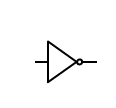
\includegraphics{./gate_not}
\end{subfigure}
\caption{Venstre: Sannhetstabell for NOT-operatoren. Høyre: Kretssymbol for NOT-port.}
\end{figure}
\end{center}

\subsubsection{AND (symbol $\land$)}
AND er en port/operasjon som tar inn to bit og gir ut en bit. AND gir ut 1 dersom begge inn-bitene er 1, ellers gir den ut 0 som vist i sannhetstabellen nedenfor.
\begin{center}
\begin{figure}[h]
\begin{subfigure}{.3\textwidth}
	\begin{tabular}{|c|c|c|}
	\hline
	$P$ & $Q$ & $P \land Q$ \\
	\hline
	0 & 0 & 0\\
	0 & 1 & 0 \\
	1 & 0 & 0 \\
	1 & 1 & 1 \\
	\hline
	\end{tabular}
\end{subfigure}
\begin{subfigure}{.3\textwidth}
	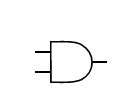
\includegraphics{./gate_and}
\end{subfigure}
\caption{Venstre: Sannhetstabell for AND-operatoren. Høyre: Kretssymbol for AND-port.}
\end{figure}
\end{center}

\subsubsection{OR (symbol $\lor$)}
OR er en port/operasjon som tar inn to bit og gir ut en bit. OR gir ut 1 dersom minst \'en av inn-bitene er 1, ellers gir den ut 0 som vist i sannhetstabellen nedenfor.
\begin{center}
\begin{figure}[h]
\begin{subfigure}{.3\textwidth}
	\begin{tabular}{|c|c|c|}
	\hline
	$P$ & $Q$ & $P \lor Q$ \\
	\hline
	0 & 0 & 0\\
	0 & 1 & 1 \\
	1 & 0 & 1 \\
	1 & 1 & 1 \\
	\hline
	\end{tabular}
\end{subfigure}
\begin{subfigure}{.3\textwidth}
	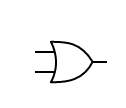
\includegraphics{./gate_or}
\end{subfigure}
\caption{Venstre: Sannhetstabell for OR-operatoren. Høyre: Kretssymbol for OR-port.}
\end{figure}
\end{center}

\subsection{Sammensatte porter}
De ulike portene som er presentert ovenfor kan kombineres til å representere en vilkårlig bineær funksjon\footnote{Det kan vises at det er tilstrekkelig med operasjonene $\neg$ og $\land$ for å oppnå dette, men det er likvel en vanlig konvensjon å beholde $\lor$ på listen over de grunnleggende logiske operasjonene.}, altså en funksjon som tar et antall bit inn og gir ut et antall bit ut med en spesifisert regel for hva som ut verdien(e) blir gitt innverdien(e). Noen slike kombinasjoner er spesielt hyppig brukt og har derfor fått egne navn og symboler. Dette inkluderer:

\subsubsection{XOR (symbol $\oplus$)}
XOR, eller exclucive or, er en operasjon/port som tar inn to bit og gir ut en bit. Denne representerer en enten/eller, altså en port som gir ut verdien 1 hvis \'en, men ikke begge inn-bitene har verdien 1. Ellers gir den ut verdien 0. XOR kan konstrueres som $P\oplus Q = (P\land\neg Q)\lor(\neg P \land Q)$. 
\begin{center}
\begin{figure}[h]
\begin{subfigure}{.3\textwidth}
	\begin{tabular}{|c|c|c|}
	\hline
	$P$ & $Q$ & $P \oplus Q$ \\
	\hline
	0 & 0 & 0\\
	0 & 1 & 1 \\
	1 & 0 & 1 \\
	1 & 1 & 0 \\
	\hline
	\end{tabular}
\end{subfigure}
\begin{subfigure}{.3\textwidth}
	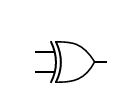
\includegraphics{./gate_xor}
\end{subfigure}
\caption{Venstre: Sannhetstabell for XOR-operatoren. Høyre: Kretssymbol for XOR-port.}
\end{figure}
\end{center}

\subsubsection{NAND (symbol $\uparrow$)}
NAND er en kombinasjon av NOT og AND. Den tar inn to bit og gir ut en bit. Siden NOT er kombinert med AND gir den alltid ut den motsatte verdien av hva AND ville gjort. NAND kan konstrueres som $P \uparrow Q = \neg(P\land Q)$. 

\begin{center}
\begin{figure}[h]
\begin{subfigure}{.3\textwidth}
	\begin{tabular}{|c|c|c|}
	\hline
	$P$ & $Q$ & $P \oplus Q$ \\
	\hline
	0 & 0 & 1\\
	0 & 1 & 1 \\
	1 & 0 & 1 \\
	1 & 1 & 0 \\
	\hline
	\end{tabular}
\end{subfigure}
\begin{subfigure}{.3\textwidth}
	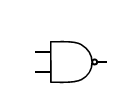
\includegraphics{./gate_nand}
\end{subfigure}
\caption{Venstre: Sannhetstabell for NAND-operatoren. Høyre: Kretssymbol for NAND-port.}
\end{figure}
\end{center}

\subsubsection{CNOT - Controlled NOT}
CNOT er en port som er veldig viktig for oss når vi kommer til kvantedatamaskiner, så derfor tar jeg med beskrivelsen av den klassiske versjonen her. Dette er det første eksempelet vi treffer på av en port med mer enn \'en ut-bit: CNOT tar inn to bit og gir ut to bit. Den første inn-biten ($x$) er kontroll-biten. Verdien av denne biten påvirker hva porten kommer til å gjøre med den andre biten ($y$). I tillegg blir kontroll-biten sendt uforandret ut av porten. Dersom kontroll-biten er 0 vil porten sende den andre biten uforandret ut, mens dersom kontroll-biten er 1 vil porten virke som en NOT-port og altså endre verdien av den andre biten før den sendes ut. Om vi sammenligner med portene som er diskutert ovenfor finner vi at den andre ut-biten bestemmes av en XOR mellom de to innbitene, altså beskrives CNOT av funksjonen $f(x,y) = (x, x\oplus y)$. Effekten av CNOT-porten er oppsummert i sannhetstabellen nedenfor.

CNOT kan konstrueres av en oppsplitting og en XOR-port som vist i figuren nedenfor. Figuren viser også kretssymbolet som vanligvis brukes for CNOT-porter.

\begin{center}
\begin{figure}[h]
\begin{subfigure}{.3\textwidth}
	\begin{tabular}{|c|c||c|c|}
		\hline
	\multicolumn{2}{|c||}{Inn} & \multicolumn{2}{|c|}{Ut} \\
	\hline
	\hline
	$x$ & $y$ & $x$ & $x\oplus y$ \\
	\hline
	\hline
	0 & 0 & 0 & 0 \\
	0 & 1 & 0 & 1 \\
	1 & 0 & 1 & 1 \\
	1 & 1 & 1 & 0 \\
	\hline
	\end{tabular}
\end{subfigure}
\begin{subfigure}{.3\textwidth}
	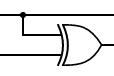
\includegraphics{./gate_cnot_comp}
\end{subfigure}
\begin{subfigure}{.3\textwidth}
	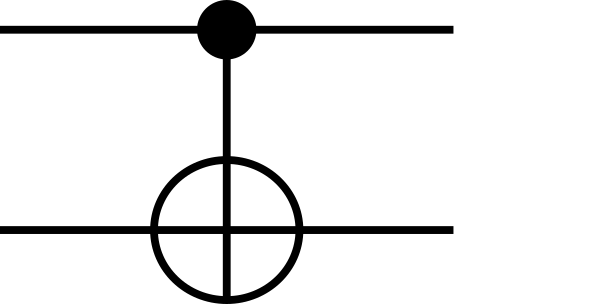
\includegraphics{./gate_cnot}
\end{subfigure}
\caption{Venstre: Sannhetstabell for CNOT-operatoren. Midten: CNOT konstruert med en oppsplitting og en XOR. Øverste inn-bit er $x$ og nederste er $y$. Tilsvarende er øverste ut-bti $x$ og nederste $x\oplus y$. Høyre: Kretssymbol for CNOT-port.}
\end{figure}
\end{center}

CNOT har den interessante egenskapen at den er reversibel. Dette er den fordi det er et en-til-en-forhold mellom hva som blir sendt ut og hva som blir sendt inn. Med andre ord: Hvis vi ser hva som kommer ut er det bare \'en mulighet for hva som ble sendt inn for å produsere dette resultatet. CNOT er dessuten sin egen invers---altså hvis vi lar det som kommer ut av en CNOT-port være innverdiene for den neste kommer vi tilbake til de bit-verdiene vi startet med.

\section{Generalisering til kvante-logiske porter}
For å lage en kvantedatamaskin trenger vi å lage en qubit-versjon av portene som er diskutert ovenfor. Vi støter da straks på en interessant utfordring: mens en klassisk bit alltid er enten 0 eller 1 vil en qubit generelt være i en superposisjon av 0 og 1. Hvordan skal vi lage sannhetstabellene når qubitene har et kontinuerlig sett av mulige verdier? La oss først få på plass litt notasjon som er nyttig i den videre diskusjonen. Nå er det tilstrekkelig for oss å jobbe med \'en basis, og der velger vi $\left\{ \left[\begin{array}{cc}1\\0\end{array}\right], \left[\begin{array}{cc}1\\0\end{array}\right] \right\}$. For å forenkle notasjonen litt kommer jeg for det meste til å skrive vektorene i bra-ket notasjon, med der basisvektorene er identifisert som
\begin{displaymath}
	|0\rangle = \left[\begin{array}{cc}1\\0\end{array}\right] \text{ og } |1\rangle =  \left[\begin{array}{cc}1\\0\end{array}\right].
\end{displaymath}
En generell qubit kan da skrives som $|a\rangle = a_0|0\rangle + a_1|1\rangle$ der $a_0^2 + a_1^2 = 1$. Når vi måler verdien av denne qubiten vil vi finne enten $|0\rangle$ eller $|1\rangle$ med sannynligheter henholdsvis $a_0^2$ og $a_1^2$. Hvis vi har mer enn en qubit å ta hensyn til, må vi ta tensorproduktet av basisvektorene for å finne den nye basisen. For eksempel er basisen for to qubit
\begin{displaymath}
	\left\{ |0\rangle\otimes|0\rangle,  |0\rangle\otimes|1\rangle,  |1\rangle\otimes|0\rangle,  |1\rangle\otimes|1\rangle  \right\}.
\end{displaymath}
For å forenkle notasjonen ytterligere innfører vi konvensjonen at $|00\rangle = |0\rangle\otimes|0\rangle$ og så videre, slik at basisen kan skrives som
\begin{displaymath}
	\left\{ |00\rangle,  |01\rangle,  |10\rangle,  |11\rangle  \right\}.
\end{displaymath}
En generell kombinasjon av to qubit kan da skrives som $|b\rangle = b_{00}|00\rangle + b_{01}|01\rangle + b_{10}|10\rangle + b_{11}|11\rangle$ der $b_{00}^2 + b_{01}^2 + b_{10}^2 + b_{11}^2 = 1$. 

\subsection{Ingen kloning-teoremet}
Vi treffer på en annen viktig forskjell mellom klassisk logikk og kvantelogikk dersom vi ønsker å klone en qubit---det vil si å lage en ekstra kopi av en qubit som er identisk med den vi har. Med klassiske bit er dette ikke noe problem. Hvis vi har en bit med en vilkårlig verdi kan vi uten problemer lage vilkårlig mange kopier av denne. Slik er det ikke i kvanteverden. Det kan vises at i det generelle tilfellet kan man ikke lage en kopi av en qubit slik at man sitter igjen med to qubit som er identiske og lik den vi startet med. Så lenge vi jobber med qubit som har en bestemt verdi er det riktignok ingen forskjell, men for å utnytte oss av fordelene som kan oppnås ved å bruke qubit i superposisjon mellom ulike verdier må algoritmene i en kvantedatamaskin lages på en slik måte at kloning av qubit er unødvendig.

Jeg vil ikke forsøke å bevise ingen kloning-teoremet her, men kun gi kvalitative argumenter som sannsynliggjør at det er riktig. En vilkårlig qubit kan som tidligere beskrevet skrives som $|a\rangle = a_0|0\rangle + a_1|1\rangle$. Dersom vi ønsker å måle verdien av qubiten vil vi aldri få noe annet enn $|0\rangle$ eller $|1\rangle$. Hvis vi kjenner $a_0$ og $a_1$ kan vi riktignok beregne sannsynligheten for hvert av de to ulike måleresultatene, men hva hvis vi har en qubit i en ukjent tilstand? Dersom vi for eksempel får resultatet $|0\rangle$ er det eneste vi kan si om koeffisientene at $a_0>0$. Vi kan altså ikke måle oss frem til hva koeffisientene $a_0$ og$a_1$ er. Men hvis vi ikke kan hente ut denne informasjonen, hvordan kan vi da lage en identisk kopi? 

\section{Matematisk beskrivelse av kvante-logiske porter}
Siden vi beskriver tilstanden til en qubit i form av en vektor er det naturlig å beskrive portene i form av matriser. Gitt en vilkårlig qubit 
\begin{displaymath}
	|a\rangle = a_0 |0\rangle + a_1|1\rangle = \left[\begin{array}{c} a_0 \\ a_1 \end{array}\right]
\end{displaymath}
Oppgaven til en port er å gjøre en operasjon på denne vektoren slik at resultatet også blir en vektor som representerer en gyldig qubit-verdi. En enkel slik operasjon er å multiplisere vektoren med en $2\times 2$ matrise, siden resultatet av denne multiplikasjonen er en vektor med samme dimensjon som vi startet med. Enhver $2\times2$ matrise vil representere en mulig port som tar en qubit som inn-verdi og gir ut en qubit som ut-verdi, men vi skal bare se på fem matriser som representerer alle en-til-en porter vi har behov for. 

\subsection{$\mathbb{I}$, $\mathbb{Z}$, $\mathbb{X}$ og $\mathbb{Y}$} 
Den enkleste porten representeres av identitetsmatrisen
\begin{displaymath}
	\mathbb{I} = \left[\begin{array}{cc}1 & 0 \\ 0 & 1 \end{array}\right]
\end{displaymath}
som ganske enkelt gir tilbake den samme qubiten vi startet med som vi kan se ved å anvende den på en vilkårlig qubit
\begin{displaymath}
	\mathbb{I}|a\rangle = \mathbb{I}(a_0|0\rangle + a_1|1\rangle)= \left[\begin{array}{cc}1 & 0 \\ 0 & 1 \end{array}\right]\left[\begin{array}{c} a_0 \\ a_1\end{array}\right] 
	= \left[\begin{array}{c} a_0 \\ a_1\end{array}\right] = a_0|0\rangle + a_1|1\rangle =  |a\rangle.
\end{displaymath}
En port som tilsynelatende gir ganske lik virkning representeres av matrisen
\begin{displaymath}
	\mathbb{Z} = \left[\begin{array}{cc}1 & 0 \\ 0 & -1 \end{array}\right].
\end{displaymath}
Anvendt på basisvektorene gir denne
\begin{align*}
	\mathbb|0\rangle &=  \left[\begin{array}{cc}1 & 0 \\ 0 & -1 \end{array}\right] \left[\begin{array}{c} 1 \\ 0 \end{array}\right]
	 =  \left[\begin{array}{c} 1 \\ 0 \end{array}\right] = |0\rangle, \\
	\mathbb|1\rangle &=  \left[\begin{array}{cc}1 & 0 \\ 0 & -1 \end{array}\right] \left[\begin{array}{r} 0 \\ 1 \end{array}\right] 
	= \left[\begin{array}{r} 0 \\ -1 \end{array}\right] = -|1\rangle.
\end{align*}
Siden en qubit $-|1\rangle$ er ekvivalent med en qubit $|1\rangle$ gir altså $\mathbb{Z}$ i likhet med $\mathbb{I}$ ingen endring så lenge vi anvender den på basisvektorer---altså på qubiter som er i en veldefinert tilstand (i motsetning til å være i en superposisjon). For $\mathbb{I}$ var den samme konklusjonen gyldig for en vilkårlig qubit, men det er ikke tilfellet for $\mathbb{Z}$. Hvis vi nå anvender denne operatoren på en vilkårlig qubit finner vi:
\begin{displaymath}
	\mathbb{Z}|a\rangle = \mathbb{Z}(a_0|0\rangle + a_1|1\rangle)= \left[\begin{array}{cc}1 & 0 \\ 0 & -1 \end{array}\right]\left[\begin{array}{c} a_0 \\ a_1\end{array}\right] 
	= \left[\begin{array}{c} a_0 \\ -a_1\end{array}\right] = a_0|0\rangle - a_1|1\rangle.
\end{displaymath}
Dette er en qubit med lik sannsynlighet for at målingen av verdien vil gi hver av de to mulighetene som qubiten vi startet med, altså
\begin{align*}
	P(|0\rangle) &= a_0^2, \\
	P(|1\rangle) &= (-a_1)^2 = a_1^2,
\end{align*}
men det er fremdeles ikke den samme qubiten. Endringen som $\mathbb{Z}$ gjør på qubiten omtaler vi som at den \emph{endrer det relative fortegnet}, og dette relative fortegnet er av stor betydning når vi ser på sammenfiltrede qubiter.

$\mathbb{X}$ og $\mathbb{Y}$ er i likhet med $\mathbb{I}$ og $\mathbb{Z}$ et par av porter som har lignende, men ikke identisk virkning på qubiter. Vi ser effekten av portene ved å anvende de på en vilkårlig qubit
\begin{align*}
	\mathbb{X}|a\rangle &= \mathbb{X}(a_0|0\rangle + a_1|1\rangle)= \left[\begin{array}{cc}0 & 1 \\ 1 & 0 \end{array}\right]\left[\begin{array}{c} a_0 \\ a_1\end{array}\right] 
	= \left[\begin{array}{c} a_1 \\ a_0\end{array}\right] = a_1|0\rangle + a_0|1\rangle, \\
	\mathbb{Y}|a\rangle &= \mathbb{X}(a_0|0\rangle + a_1|1\rangle)= \left[\begin{array}{cc}0 & 1 \\ -1 & 0 \end{array}\right]\left[\begin{array}{c} a_0 \\ a_1\end{array}\right] 
	= \left[\begin{array}{c} a_1 \\ -a_0\end{array}\right] = a_1|0\rangle - a_0|1\rangle.
\end{align*}
Hvis vi først setter $a_0=1, a_1=0$ eller $a_0=0, a_1=1$ for å studere virkningen på basisvektorer ser vi at både $\mathbb{X}$ og $\mathbb{Y}$ er en slags NOT-port---de endrer $|0\rangle$ til $|1\rangle$ og motsatt. Forskjellen på de to portene er at dersom vi har en qubit som er i en superposisjon vil $\mathbb{Y}$ endre det relative fortegnet, mens $\mathbb{X}$ ikke gjør det.

\subsection{Hadamard-porten $\mathbb{H}$}
Den viktigste porten som virker på \'en qubit er Hadamard-porten
\begin{displaymath}
	\mathbb{H} = \ipsqrt \left[\begin{array}{cc}1 & 1 \\ 1 & -1 \end{array}\right].
\end{displaymath}
Faktoren $\ipsqrt$ er tatt med for å beholde normaliseringen av qubitene---altså slik at kvadratsummen av koeffisientene ikke endres. For å se hvorfor Hadamard-porten er viktig studerer vi hvilken effekt den har på basisvektorene:
\begin{align*}
	\mathbb{H}|0\rangle &= \ipsqrt\left[\begin{array}{cc}1 & 1 \\ 1 & -1 \end{array}\right]\left[\begin{array}{c} 1 \\ 0\end{array}\right] 
	= \ipsqrt\left[\begin{array}{c} 1 \\ 1\end{array}\right] = \ipsqrt(|0\rangle + |1\rangle), \\
	\mathbb{H}|1\rangle &= \ipsqrt\left[\begin{array}{cc}1 & 1 \\ 1 & -1 \end{array}\right]\left[\begin{array}{c} 0 \\ 1\end{array}\right] 
	= \ipsqrt\left[\begin{array}{c} 1 \\ -1\end{array}\right] = \ipsqrt(|0\rangle - |1\rangle).
\end{align*}
Vi ser altså at når Hadamard-porten virker på en qubit som er i en veldefinert tilstand blir resultatet en qubit som er i en superposisjon med lik sannsynlighet for å bli målt til hver av de to ulike verdiene.